Using the thesis work might not be totally self explanatory.
Here follows a couple of walk-through sections on how to use the different parts.
First thing to do in every scenario is to run the init{\_}script.m.
This ensures that folders are added to the MATLAB workpath.

\subsection{Running hexapod Model}
For running the hexapod as a model the file Control/DevelopmentModel.slx can be used.
This file contains a Model of the hexapod built up by the different library files and a controller built up similarly.
Running the combination of the two is done by basically pressing play and SimMechanics should provide visual results.
If there is a desire to change the hard-coded input to the controller one can change this inside the controller block 2 levels down.
All changes to main controller and IK should be avoided inside this file.
Those changes are better done in the library files.

\subsection{Running Code Generation to the hexapod}
First assemble the power to the hexapod.
Connect the battery to the battery voltage monitor device to be able to monitor battery voltage.
The monitor device will beep temporary when connected.
When battery voltage is to low the device will start beeping continuously (charge the battery).
Also connect the battery to the connection bringing power to BeagleBone Black, ArbotiX and servos.
The BeagleBone gets powered directly but in order to power ArbotiX and servos the switch on the back of the hexapod has to be switched.

Start the file Control/CodeGenerationSetup.slx.
This files provide two options, run in external mode or deploy to hardware.
Running in external mode (play button) provides the ability to monitor signals with scopes in Simulink but needs the BeagleBone connected to the computer by USB.
Deploy to hardware (blue deploy button) allows for no wire connection but do not supply scope data.

Power on the remote first after the code has started running to avoid communication being off-sync.
When deployed to hardware the script StartBB and StopBB can be used to start/stop the program without having to recompile code.

\newpage
\subsection{Using the remote}

A picture of the remote can be seen in Figure \ref{fig:commander}.
Description of each button is described in Table \ref{tab:remotecontroll}.



\begin{figure}[h!]%float objekt h-här h!-verkligen här t-toppen
\centering%centrerar bilden på sidan
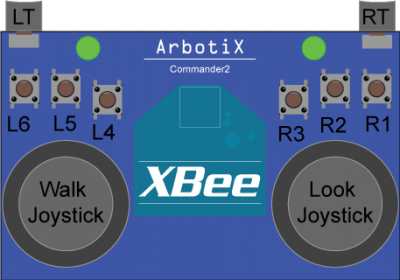
\includegraphics[width=0.7\textwidth]{Commander.png}%0.9 textbredder
\caption{Location on the different controls on the remote.}%skapa bildtext
\label{fig:commander}%tag label på bilden
\end{figure}


\setlength{\extrarowheight}{5pt}
%%Command for writing data to all of the servos
\begin{table}[h!]
\centering%centrerar bilden på sidan
\begin{tabular}{|l|l|}
\hline Name 					&   Description			\\ 
\hline WalkH $\leftrightarrow$	& 	Strafe left/right	\\ 
\hline WalkV $\updownarrow$ 	&   Move forward/back 	\\ 
\hline LookH $\leftrightarrow$	& 	Rotate left/right 	\\  
\hline LookV $\updownarrow$		&   N/A					\\ 
\hline LT&      Lower the body		\\
\hline RT& 	    Rise the body		\\  
\hline L6&      Normal walking		\\ 
\hline L5&      Experimental walk patterns with constraints\\
\hline L4&      N/A					\\
\hline R3& 	    N/A					\\  
\hline R2&      N/A					\\ 
\hline R1&      Balancing mode    	\\
\hline 
\end{tabular} 
\caption{Description of the remote control.}%skapa bildtext
\label{tab:remotecontroll}%tag label på bilden
\end{table}


